%%
% TUM Corporate Design LaTeX Templates
% Based on the templates from https://www.tum.de/cd
%
% Feel free to join development on
% https://gitlab.lrz.de/tum-templates/templates
% and/or to create an issue in case of trouble.
%
% tum-article class for scientific articles, reports, exercise sheets, ...
%
%%

\documentclass[twocolumn]{tum-article}
%\documentclass[twocolumn, german]{tum-article}
%\documentclass[times, twocolumn]{tum-article}
%\documentclass[times]{tum-article}
%\documentclass{tum-article}

%\usepackage{lipsum}
\usepackage{amsmath}

\title{Analysis of the 2014 Passenger Flight Network}
\author{Felix Paul Niemeyer\authormark{1},
	Saicharan Kumar\authormark{2}}
% Author 3\authormark{1}\orcid{0000-0000-0000-0000}}

% if too long for running head
\titlerunning{TUM Article}
\authorrunning{Author 1 et al.}

%\email{niemeyer.felix@tum.de}

\affil[1]{felix.niemeyer@tum.de, MiM}
\affil[2]{saicharan.kumar@tum.de, MiM}

\date{Handed in on 19.02.2020}

% for the equation stuff 
\DeclareMathOperator{\avgFlow}{avgFlow}
\DeclareMathOperator{\patronage}{patr}
\DeclareMathOperator{\flow}{flow}
\DeclareMathOperator{\weight}{weight}
\DeclareMathOperator{\PNWS}{PNWS}
\DeclareMathOperator{\NOE}{NOE}
\DeclareMathOperator{\degree}{degree}
\DeclareMathOperator{\flowSum}{flowSum}
\DeclareMathOperator{\flowDeviation}{flowDeviation}
\DeclareMathOperator{\flowDiff}{flowDiff}
\DeclareMathOperator{\Largeness}{largeness}
\DeclareMathOperator{\Potential}{potential}
\DeclareMathOperator{\WEVC}{WEVC}
\DeclareMathOperator{\Nodes}{Nodes}

\begin{document}

\maketitle

\begin{abstract}
In this case study we are looking at a dataset about air travel in 2014. 
We implement some mechanisms to clean the data, as well as mechanisms to enrich this dataset with information we query from wikidata.
We estimate some missing data.
Starting from there, we analyze some network characteristics for the whole network as well as airline-specific sub-networks.
We compare airline-specific networks and find relations between their network's characteristics and their business model.
We propose one metric that plays a role in forecasting whether a cooperation between two airlines is advantageous and use this metric to generate an alliances landscape.
We compare it's predictive correctness to the real world, criticise it and present one promising further approach. 
\end{abstract}

\section{Data Description}
The network analysis is based on dataset from openflights.org. 
It describes passenger flight connections between airports in the year 2014. 
The data includes, which airline each connection is operated by.
The data comes in three tables: airports, routes and airlines. 
The airports table has entries for every airport with the following useful information: \\
- airport id\\
- iata and icao codes\\
- geographic coordinates\\
- country and region\\

The routes table lists an entry for each connection between two airports that was operated by an airline sometime in the year 2014. It does not contain any information about flight frequencies or passenger volume. The airline table lists airlines associated with their name and some information we do not need like country or call sign. \\

We are loading these files into an SQLite database for easier handling. 
We apply some queries for cleaning the data, e.g. removing routes operated by unknown airlines or filling in airport ids in routes where only iata or icao code is used to refer to a source or destination airport. \\

All the data-setup can be accomplished by running a single script.
This script and also all other code we have written for this project can be found in a public repository on GitHub\cite{repository}.

\section{Data Enrichment \& Estimation}
After cleaning up the data, there are 3139 airports. 
Interpreting the data as a graph gives us a multi-edge directed graph.
Looking at the degree distribution in Figure~\ref{fig:degree_distribution}, the alternating characteristic of degrees strikes the eye. It comes from the fact, that it's very uncommon for a connection between airports to exist only in one direction. Thus, there is much fewer nodes with odd degrees than than with even degrees. 

When we disregard odd degrees, the seemingly linear distribution on a log log scale becomes apparent. Using least square (scipy.optimize.curve\_fit), we optimize parameters $c$ and $\gamma$ as you can see in Figure~\ref{fig:degree_distribution_curves}

\begin{figure}
	\centering
	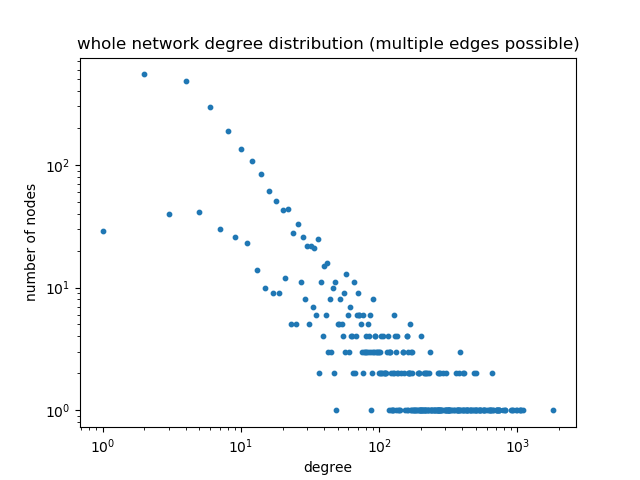
\includegraphics[width=76mm]{imgs/results/degree_distribution_incl_odd_degrees.png}
	\caption{
The degree distribution of the network on a log log scale }
	\label{fig:degree_distribution}
\end{figure}

\begin{figure}
	\centering
	\includegraphics[width=76mm]{imgs/results/degree_distribution_curve_manual.png}
	\caption{
Looking at even degrees only. Trying least square curve fitting to find suitable parameters for power law distribution function $f(x) = a * x^{-\gamma}$}
	\label{fig:degree_distribution_curves}
\end{figure}

Besides the main subgraph, that includes 3113 nodes, there are 6 small disconnected ones with only a couple of nodes.
One with 10 nodes for example, Figure~\ref{fig:new_caledonia}, consists only of airports that are located in New Caledonia, an archipelago in the Pacific Ocean. 
\begin{figure}
	\centering
	\includegraphics[width=76mm]{imgs/new-caledonia-subgraph.png}
	\caption{Airports of New Caledonia drawn on a map}
	\label{fig:new_caledonia}
\end{figure}

In order to enable us to do more meaningful analysis, we enrich the dataset with additional information. We chose the airport patronage and found out, that we can get this data from Wikidata. 
For 1956 of the 3139 airports from the dataset, we can find patronage data from Wikidata. We can also get an impression about the regional differences of data availability, by looking at the percentage of airports for which Wikidata yields a patronage in Table~\ref{tab:patr_av_most_airports} and Table~\ref{tab:patr_av_worst}.
\begin{table}[h]
	\centering
	\caption{patronage data availability on Wikidata for countries with the most airports}
	\label{tab:patr_av_most_airports}
	\begin{tabular}{|l|c|c|}
		\hline
		Country & Airports & patronage present \\ \hline
		United States & 539 & 34.1\%\\
		China & 173 & 95.4\%\\
		Canada & 142 & 48.6\%\\
		Brazil & 122 & 93.4\%\\
		Australia & 113 & 77.0\%\\
		Russia & 103 & 96.1\%\\
		India & 70 & 92.9\%\\
		Indonesia & 63 & 60.3\%\\
		Japan & 62 & 82.3\%\\
		Mexico & 56 & 92.9\%\\
		France & 55 & 96.4\%\\ \hline
	\end{tabular}
\end{table}
\begin{table}[h]
	\centering
	\caption{Worst patronage data availability on Wikidata}
	\label{tab:patr_av_worst}
	\begin{tabular}{|l|c|c|}
		\hline
		Country & Airports & patronage present \\ \hline
		Venezuela & 23 & 4.3\%\\
		Bahamas & 17 & 5.9\%\\
		Chile & 16 & 6.3\%\\
		Ecuador & 14 & 7.1\%\\
		Ethiopia & 13 & 7.7\%\\ 
		Mozambique & 10 & 10.0\%\\
		Cuba & 9 & 11.1\%\\
		Kenya & 16 & 12.5\%\\
		Namibia & 8 & 12.5\%\\
		Madagascar & 13 & 15.4\%\\
		Algeria & 26 & 19.2\%\\ \hline
	\end{tabular}
\end{table}
We need to distinguish between monthly and yearly values and we extrapolate 2014 data from close years in case there is no data for the year 2014. 
In order to populate the remaining nodes with reasonable patronages as well, we tried different techniques. 


First we used data about runway surfaces that we found on ourflights.org. 
We summed up the surfaces of runways for every airport and then calculated the average ratio between total runway surface area and patronage of airports where both data points were present, in order to predict patronage for airports without patronage data but with runway surface data based on this average ratio. 
For the still remaining >1000 airports without patronage we would then apply a default value that equals the average of the smallest 1\% of airports with patronage data from Wikidata. 
The runway data turned out to be very unclean and unreliable. Water runways and other quirks were distorting the predictions. 

Inspired by Prof. Ikonnikova's advice during the presentation we switched to estimating the remaining airport patronages by looking at neighboring airports with patronage data. The Algorithm can be seen in Listing~\ref{lst:patronage_estimation_algorithm}.
\begin{lstlisting}[language=Python, caption={Patronage estimation algorithm, that uses neighboring airport's patronage data}, label=lst:patronage_estimation_algorithm]
G = loadEntireNetwork()
pr = -1 #previous remaining
r = 0   #remaining
while r != pr:
  pr = r
  r = 0
  ep = {} #estimated patronages
  for apid in G.nodes:
    node = G.nodes[apid]
    if node["patronage"] == None:
      neighbors = G.neighbors(apid) 
      deg = G.degree(apid)
      sum = 0
      count = 0
      for nid in neighbors: 
        n = G.nodes[nid]
        npatr = n["patronage"]
        ndeg = G.degree(nid) 
        if npatr != None: 
          sum += deg * npatr / ndeg
          count += 1
      if count == 0:
        r += 1
      else:
        avg = sum / count
        ep[apid] = avg 
  for apid in ep: 
    node = G.nodes[apid]
    node["patronage"] = ep[apid]
\end{lstlisting}
This second approach yields much nicer estimations, as we will see after estimating the flows between airports. 

After estimating missing patronage data by looking at neighboring airports patronages, 14 airports without patronage remain. These must be in airports in disconnected subgraphs, because the algorithm would eventually reach them and assign a patronage otherwise. Investigations confirm that. We disregard these few data-less airports from disconnected subgraphs in the following analyses and thus end up with a network of 3125 airports. 

The flows are estimated by choosing reasonable initial values and then applying corrections iteratively to approach a situation where the sum of the estimated elows for each airport equal its patronage value.
The average initial values for an edge between airport $p$ and $q$ is chosen as: 


\begin{equation}
\avgFlow(pq) = \dfrac{\patronage(p) * \patronage(q)}{\degree(p) * \degree(q)}
\end{equation}
Remember that we are handling a multi-edge directed graph here. 
\begin{equation}
E = \{(pql) | \exists\ \text{route from}\ p\ \text{to}\ q\ \text{by}\ l\}
\end{equation}
where $p$ and $q$ are airports and $l$ is an airline.
Let us introduce a function $E(pq)$ that returns all edges between $p$ and $q$ disregarding the direction and operating airline. 
\begin{equation}
E(pq) = \{pql | \exists_{l \in L}:pql \in E \lor qpl \in E\}
\end{equation}
where $L$ is the set of airlines.

And let us introduce the function $E(p)$ that returns all edges from and to an airport $p$ by every airline: 
\begin{equation}
E(p) = \{rsl | (r=p \lor s=p) \land \exists_{l \in L}:rsl \in E \}
\end{equation}
The Edges of the graph are thus triplets of a source airport, destination airport and an airline.
There may be multiple edges between two airports pointing in different directions and/or operated by different airlines.
We could assume an equal distribution of the flows among the edges. But we chose trying to be closer to reality by weighting the flow of an edge between two airports $p$ and $q$, that is operated by airline $l$, by the geometric mean of the number of edges airline $l$ operates at airport $p$ and number of edges airline $l$ operates at airport $q$: 
\begin{equation}
\begin{aligned}
&\flow(pql) =\\
={}&\avgFlow(pq)  
* \NOE(pq) 
* \weight(pql) 
\end{aligned}
\end{equation}
where $\NOE(pq)$ is the number of edges between airport $p$ and $q$ and $\weight(pql)$ is defined as follows: 
\begin{equation}
\begin{aligned}
&\weight(pql) = \dfrac{\sqrt{\degree_{l}(p) * \degree_{l}(q)}}{\PNWS(pql)}
\end{aligned}
\end{equation}
where the $\PNWS(pq)$ (Pre Normalization Weight Sum) is just the sum of the non-normalized weights of all the routes from different airlines used to normalize the weights. 
\begin{equation}
\begin{aligned}
&\PNWS(pq) = \\
={}&\displaystyle\sum_{rsm \in E(pq)}(\sqrt{\degree_{m}(r) * \degree_{m}(s)})
\end{aligned}
\end{equation}
where $\degree_l(p)$ is the degree of airport $p$ in airline $l$'s subgraph, i.e. number of edges from and to airport $p$ operated by airline $l$.

The ratios we choose here will stay intact over the course of the iterations in the next part of the algorithm.
In every iteration, we traverse all airports and for every airport we calculate the sum of current flow values of all routes. 
\begin{equation}
\begin{aligned}
\flowSum(p) = \displaystyle\sum_{pql \in E \cup pu \in E}\flow_{pql}
\end{aligned}
\end{equation}
Then, for each airport we calculate the difference between its patronage and the current sum of flows.
\begin{equation}
\begin{aligned}
\flowDiff(p) = \patronage(p) - \flowSum(p) 
\end{aligned}
\end{equation}
With this information given, we can now calculate for every edge $pql$ the change in its flow. 
\begin{equation}
\begin{aligned}
\forall_{pql \in E(p)}: & \\
& \Delta \flow(pql) = & \\ 
& ={} \dfrac{\flow(pql)}{\flowSum(p)}\flowDiff(p) \\
& +{} \dfrac{\flow(pql)}{\flowSum(q)}\flowDiff(q) \\
\end{aligned}
\end{equation}
and the more perfect flows for the edges and starting point for the next iteration are
\begin{equation}
\begin{aligned}
\forall_{pql \in E(p)}: & \\
& \flow'(pql) = \flow_{abo} + \Delta \flow(pql)
\end{aligned}
\end{equation}

In order to look at the results of this algorithm we introduce a measure 
\begin{equation}
\flowDeviation(p) = ln\left(\dfrac{\flowSum(p)}{\patronage(p)}\right)
\end{equation}
It expresses how well the sum of estimated flows match the patronage, that we know for the airport. If the flows are half the patronage the absolute value of $\flowDeviation$ will be the same as when the current flows are twice the actual patronage number. 
We compare the results between estimating the patronages based on the runway sizes Figure~\ref{fig:flow_deviation_runway} and estimating the patronages based on neighboring airports Figure~\ref{fig:flow_deviation}. 
The blue line shows the $\flowDeviation$ distribution of the initial flow values.
The other lines show the $\flowDeviation$ distribution after the first couple of iterations and after the final iteration. 
In the case of patronage estimations based on neighboring airports, we see that the $\flowDeviation$ distribution after the 120th iteration comes very close to $y=0$ which is also reflected by the $sum(abs)$ in the legend, which is the sum of the absolute value of $\flowDeviation$ over all airports which is $0.94$ in this case.

The bad results of the estimations when estimating patronage values from runways stem from constellations like in Figure~\ref{fig:impossible_flows}, when choosing flows to match the patronage values are impossible. 
The constellation that accounts for $>0.88$ of the $\flowDeviation$ sum $0.94$ in the scenario where patronages are estimated based on neighboring airports is shown in Figure~\ref{fig:worst_flow_fit}. 
The patronage of both airports comes from Wikidata. After further investigation it turns out to be probable, that there should be a connection between Arvidsjaur Airport and Stockholm-Arlanda Airport, which is not present in the data set. 

\begin{figure}[h]
	\centering
	\includegraphics[width=76mm]{imgs/flow_estimation_runway_approach_deviation.png}
	\caption{
Estimated flows when estimating patronage based on the runway size and a default value}
	\label{fig:flow_deviation_runway}
\end{figure}

\begin{figure}[h]
	\centering
	\includegraphics[width=76mm]{imgs/results/flow_estimation_120_iterations.png}
	\caption{
Estimated flows when estimating patronage based on neighboring airport's patronage}
	\label{fig:flow_deviation}
\end{figure}

The complete algorithm for passenger flow estimation can be found in the repository: ./scripts/estimate-passenger-flows.py

\begin{figure}[h]
	\centering
	\includegraphics[width=76mm]{imgs/runway-based-estimation-problem.png}
	\caption{Worst situation in the scenario, where patronages are estimated based on runways and a default value: 
For Qaanaaq Airport there was no patronage data from Wikidata and no runway information. That's why it ended up with the default patronage value 1523. In this constellation it is impossible to choose passenger flows that even remotely satisfy the the patronages of airports with ids 10 and 5446}
	\label{fig:impossible_flows}
\end{figure}

\begin{figure}[h]
	\centering
	\includegraphics[width=76mm]{imgs/results/ego_graph_730.png}
	\caption{Worst situation in the scenario, where patronage is based on neighboring airport's patronage: 
Arvidsjaur Airport is only connected to Lycksele Airport but has a more than twice as high patronage than Lycksele Airport}
	\label{fig:worst_flow_fit}
\end{figure}



\section{Basic Network Analysis}
Initially, we would like to analyze the entire worldwide airline network, and provide some insights regarding the airline industry.
Since a particular route could be provided by multiple airline companies, the final network that we come up with is a multiple directed network.
After enrichment the attributes of each edge in this network include both the geometrical distance and the average passenger flow of that route (edge). 
As we can see from the Table~\ref{Tab:distance_metrics}, the diameter of the entire network is given along with the total distance of the routes and the average distance of routes in a network.  

\begin{table}[ht]	
\begin{center}
 \begin{tabular}{| c | c | c |}
 \hline
 \textbf{Diameter} & \textbf{Total Dist.} & \textbf{Average Dist.} \\ 
 \hline
 18834 & 126681574 & 1889.72 \\
 \hline
 \end{tabular}
\caption{Distance metrics of the network in km}
\label{Tab:distance_metrics}	 
\end{center}
\end{table}

For a multi directed graph, most centrality measures except degree centrality (Figure~\ref{fig:degree_centrality}) are not defined. 

\begin{figure}
        \centering
        \includegraphics[width=80mm]{imgs2/results/degree_centrality_whole_network.png}
        \caption{
The degree centrality of the entire network}
        \label{fig:degree_centrality}
\end{figure}

The degree centrality is given by the formula:
\begin{equation}
	Degree Centrality=d_i/(n-1)
\end{equation}

However, a multi directed graph can be converted to a directed graph, by merging the edges. 

Just by analyzing the graph, we can say that the degree centrality distribution is following the power law distribution.

\section{Airline Subgraph Analysis \& Comparison}

Airline networks can be mainly divided into two different types of networks. Full service airlines which are also called legacy carriers, and low cost airlines or low cost carriers.  
Full service airlines generally provide free baggage allowance, meals, drinks, seat selection and in-flight entertainment at no extra charge.
Low cost carriers will usually collect ancillary revenue for all or most of the these amenities.
Most of the time, low cost carriers operate in a specific regions.
These specific regions could be within countries, within continents, or within specific parts of the continents.

\begin{figure}
        \centering
        \includegraphics[width=80mm]{imgs2/united_airline_network.png}
        \caption{
Network of United Airlines}
        \label{fig:united_airline}
\end{figure}

\begin{figure}
        \centering
        \includegraphics[width=80mm]{imgs2/american_airline_network.png}
        \caption{
Network of American Airlines}
        \label{fig:american_airline}
\end{figure}



Long haul low cost carriers are provided by very few carriers in the world, as it is not feasible to offer long routes with low cost and also high frequency, according to Robert L. Candall, former CEO of American Airlines.\cite{long_haul_lcc_model}
The only example we have of a long haul low cost carrier is Norwegian Airlines, as they offer flights from Scandinavia to different cities in the United States.
But this is more an exception, than the norm. For the long haul low cost carriers to survive and adapt, they must continue to innovate. Their business models should focus on three new emerging carrier types: network, product and price Specialist, according to John G.Wensveen and Ryan Leick.\cite{long_haul_lcc_new_model}


Before we look at the differences in the network parameters of these two types of airlines, there are major differences in the network architecture itself.
While the major full service airlines often have the network type of "Hub and Spoke", the low cost carriers are known to have "Point to Point" network type, according to research by Cook G.N and Goodwin, J.\cite{airline_network_comparison}
This "Hub and Spoke" network connection can be seen in the network graph of United Airlines and American Airlines given in Figure~\ref{fig:united_airline} and Figure~\ref{fig:american_airline} respectively. These two airlines are prime example of full service airlines. 


Similarly we see the "Point to Point" Network in low cost carriers like Ryan Air in Figure~\ref{fig:ryan_air} and Southwest Airlines in Figure~\ref{fig:southwest_airline}.

\begin{figure}
        \centering
        \includegraphics[width=80mm]{imgs2/ryan_air_network.png}
        \caption{
Network of Ryanair}
        \label{fig:ryan_air}
\end{figure}

\begin{figure}
        \centering
        \includegraphics[width=80mm]{imgs2/southwest_airline_network.png}
        \caption{
Network of Southwest Airlines}
        \label{fig:southwest_airline}
\end{figure}


We can also notice these major differences by analyzing various parameters for airline subgraphs.
As shown in Table~\ref{Tab:distance_airlines}, we can see that the full service airlines like United Airlines, American Airlines and Delta Airlines, offer routes over really long distances.
That is the reason why the geometric distance diameters of these airline networks are easily over 12000 km.
On the other hand, low cost carriers offer routes within a certain region, such as within Europe (Ryan Air) or within the United States (Southwest Airlines).
And as expected, the diameter of these airline networks are below 4000 km. 


The differences are also apparent when we look at the mean geometric distance of all the routes offered by a particular airline.
Full service carriers show an average route distance of around 2300 km, while the low cost carriers show that their average route distance is about 1400 km, which is significantly lower.


We would also like to point out the case of China Southern Airlines and China Eastern Airlines.
The diameter of those two airlines is as large as the one of United or Delta Airlines. 
But when we look at the mean distances of the those two Chinese airlines, they are only around 1400 km, which is common for airlines like Ryanair or Southwest Airlines.
This discrepancy can be explained by analyzing the median geometric distance of these networks.
These Chinese Airlines have a median of around 1100 km, which means they have a lot of routes which are within China region only. 
And looking at the full network, we can also say that, the main reason their diameter is over 12000 km is because they had recently started to offer few routes to countries like Canada, United States and Germany.
Although these are large distances, due to the high number of local routes within China, the mean route length of this network, turns out to be much lesser and comparable to low cost carriers. 

\begin{table}[h]
\begin{center}
 \begin{tabular}{| l | r | r | r |}
 \hline
 \textbf{Airline} & \textbf{Mean} & \textbf{Median} & \textbf{Diam.} \\ 
 \hline
 United & 2353.69 & 1393 & 12979 \\
 \hline   
 American & 2321.23 & 1371 & 14076 \\
 \hline   
 Delta & 2352.17 & 1341 & 13581 \\
 \hline   
 Ryan Air & 1490.21 & 1435 & 3698 \\
 \hline   
 Southwest & 1398.37 & 1267 & 3757 \\
 \hline   
 Air Asia & 1328.57 & 1254 & 2914 \\
 \hline   
 Ch. Southern & 1459.95 & 1127 & 11637 \\
 \hline   
 Ch. Eastern & 1427.81 & 1075 & 11896 \\
 \hline
 \end{tabular}
\caption{Mean, median and diameter of subgraphs of major airlines (all numbers in km)}
\label{Tab:distance_airlines}
\end{center}
\end{table}

\begin{table}[h]
\begin{center}
 \begin{tabular}{| l | r | r |}
 \hline
 \textbf{Airline} & \textbf{Mean Flow} & \textbf{Median Flow} \\ 
 \hline
 United & 85159 & 43286 \\
 \hline
 American & 67983.40 & 47185 \\
 \hline
 Delta & 76345.95  & 47123 \\
 \hline
 Ryan Air & 31268.60 & 26857.50 \\
 \hline
 Southwest & 65692.70  & 61590 \\
 \hline
 Ch. Southern & 53100  & 43729.50 \\
 \hline
 Ch. Eastern & 52610.60  & 43294 \\
 \hline
 \end{tabular}
\caption{Passenger flow of major airlines}
\label{Tab:passenger_flow_airlines}
\end{center}
\end{table}

\begin{figure}
        \centering
        \includegraphics[width=80mm]{imgs2/results/eigenvector_centrality_distribution.png}
        \caption{
Eigenvector centrality distribution}
        \label{fig:eigen_distr}
\end{figure}

\begin{figure}
        \centering
        \includegraphics[width=80mm]{imgs2/results/closeness_centrality_distribution.png}
        \caption{
Closeness centrality distribution}
        \label{fig:closeness_distr}
\end{figure}


\begin{figure}
        \centering
        \includegraphics[width=80mm]{imgs2/results/geometrical_distance_distribution.png}
        \caption{
Geometrical distance distribution}
        \label{fig:geometric_distr}
\end{figure}

Figure~\ref{fig:geometric_distr} provides us the geometric route distance distribution for airlines United, Lufthansa, Ryanair and Southwest. Here too, there is an apparent distinction between the full service airlines and the low cost carriers. 	
Ryanair and Southwest offer so many routes around 1000 km range, that the peak of their distribution is also around that value.
And of course, their routes stop at a maximum distance of around 4000 km. 
Looking at the full service carriers, though the global peak of the distribution of United and Lufthansa is also around the same distance of 1000 km, we can see that there is a second small peak at around 6000 km. This is to a big extetent caused by transatlantic flights between United States and Europe. 
Both of these airlines offer a considerable number of these routes, that it shows in the distribution curve distinctly. 


The centrality distributions (both eigenvector and closeness) of these four airlines also provide us with deep insights into their route network. 
We see that in both the Figures~\ref{fig:eigen_distr} and ~\ref{fig:closeness_distr}, Ryan Air and Southwest have more airports with higher centrality value.
We could say that the centrality of their network is distributed across many airports, instead of relying on few airports with really high centrality values. 
The scenario of having few airports with really high centrality value is seen in the case of full service airlines Lufthansa and United Airlines. They have a high number of airports with low centrality, and a few select airports with high centrality values.
If we look at the network diagram that was previously shown in Figure~\ref{fig:united_airline}, it is apparent that these high centrality airports are basically the hubs of these networks.  

\section{Airline Cooperation Potential}

The possibility to provide convenient on-line connections to clients is an important factor that drives welfare gains through airline cooperation according to E. E. Bailey and D. Liu \cite{airline_consolidation_and_consumer_welfare}.

In this paper Bailey et al. emphasize the importance of network effects for airline competition. They mention Carlton, Landes and Posner \cite{costs-and-benefits-of-airline-mergers}, who found out, that when there is an intermediate stop on a trip, consumer welfare is higher, if both segments are operated by the same airline. 
"The connection and navigation times within the hub airport are shorter and the hassle is less than with a change of carrier" \cite{airline_consolidation_and_consumer_welfare}. 
Think for example about the hassle that arises if you have booked two segments independently and you miss the second flight due to a delay of the first flight. 

There is a welfare gain, when a connection from A to B could previously only be achieved by booking a flight with two different airlines, can now be achieved by booking two flights from a single airline within one ticket. 
It is better for a consumer, to buy one ticket for a flight \mbox{A$\rightarrow$B$\rightarrow$C} from a single airline 
Than buying two tickets for \mbox{A$\rightarrow$B} and \mbox{B$\rightarrow$C} from two distinct airlines.

We construct a simple but powerful metric that captures this welfare gain for a potential merge of two airlines $l$ and $m$. 

First, we define a $\Largeness_{2}$ of an airline, that is the sum of all length-2 flights operated by this airline, weighted by the "popularity" of the two connected airports.
We weight by the "popularity", because the welfare gain from a possibility to book a length-2 flight with a single ticket scales with the demand for this connection. 

\begin{equation}
\begin{aligned}
 & \Largeness_{2}(l) = \\
= & \displaystyle\sum_{\substack{p,r \in P \\ \exists_{q}: pql \in E \and qrl \in E}}: \sqrt(\patronage(p) * \patronage(r))
\end{aligned}
\end{equation}

To assess the potential of a merge, we divide the Largeness of the joint airline network by the sum of the Largenesses of the separate airline networks. 

\begin{equation}
\begin{aligned}
& \Potential(l,m) = \\
={} & \dfrac{\Largeness_{2}(l \cup m)}{\Largeness_{2}(l) + \Largeness_{2}(m)} 
\end{aligned}
\end{equation}

Imagine the merge of two airlines yields many new 2-segment flight routes (look at the example in Figure~\ref{fig:potential-example}). If there is already a big overlap between the networks, $\Potential(l,m)$ might even be $< 1$ and thus discourage a merger or cooperation\footnote{this aspect of the $\Largeness$ metric might deserve criticism. See section "Outlook" for details.} 

\begin{figure}
	\centering
	\includegraphics[width=76mm]{imgs/potential-example.png}
	\caption{
The merger of the blue and green airline networks yields six additional 2-segment connections}
	\label{fig:potential-example}
\end{figure}

Because airlines from the same alliance can offer 2-segment flights in one ticket just as merged airlines can, this metric is also applicable for cooperation between airlines or alliance forming. 


With this metric at hand, we can give answers to questions like: 

"Which alliance should airline X join?"

"Which airlines should form alliances?" 


We don't linger on small questions like this and jump right into reorganizing the airline alliance landscape\footnote{this wording is supposed to be funny and caricaturing. Obviously, the factors that lead to forming of alliances are incredibly diverse ranging from historical reasons to interpersonal reasons, and we do not expect that a generated alliance landscape would exactly return the real alliances landscape, that we observe today. But we are looking for meta similarities, that describe the characteristics of an alliance landscape. As we assume $\Largeness_{2}$ to be an important factor in alliance formation, we a curious to find out which similarities we will be able to spot}. We implemented an algorithm that merges one airline with another, until only $N$ are left. In each step, the two airlines $l$ and $m$ are merged, that have the highest $\Potential$.

We plot the result on a world map (Figure~\ref{fig:generated-alliance-map}) and compare it to the real alliance landscape (Figure~\ref{fig:real-alliance-map}. A remarkable similarity between the generated alliance landscape and the real one, is that one big alliance (the green alliance) is covering a lot of flights between the US, Europe and China, but is not much active in South America, South Africa, Australia or New Zealand. It also does not operate much in Canada in both the generated and real alliances landscape. 
As expected, there are also differences: For example the generated alliance Landscape suggests Spanish speaking South American Countries to be in the same alliance and have Brazilian operators that are mostly part of the green alliance, while in real life Buenos Aires is tied to the Skyteam while Brazil gets supplied by a mix of alliances. Japan for example belongs to Staralliance in the real world while in the generated landscape it's a part of the green alliance. 

\begin{figure}[t]
	\centering
	\includegraphics[width=76mm]{imgs/generated-alliance-map.png}
	\caption{
The generated alliance landscape. Different colors mean different alliances. Green, Blue, Purple, Yellow. (Be aware, that by layering the networks of the different alliances on top of each other and routes in a higher layer covering the lower levels, the perception might be distorted.)}
	\label{fig:generated-alliance-map}
\end{figure}

\begin{figure}[t]
	\centering
	\includegraphics[width=76mm]{imgs/real-alliance-map.png}
	\caption{
The real alliance landscape. Skyteam(green), Staralliance(blue), Oneworld(purple), Vanilla(yellow)}
	\label{fig:real-alliance-map}
\end{figure}

\section{Outlook: Improving the metric}
The $\Largeness_{2}$ metric could be improved. Right now, when two airlines have the same 2-segment connections, after joining the network, those connections will be counted only once. There is no clear reasoning why these overlaps should discourage a merger. 

A very promising different approach to capturing welfare that arises from additional single-ticket multi-segment flights through a merger or cooperation between airlines, is to look at the sum of the product of the weighted eigenvector centralities of common airports of the two merge candidates. 

\begin{equation}
\begin{aligned}
& \Potential_{\WEVC}(l, m) = \\
 = & \sum_{p \in \Nodes(l \cap m)}: \WEVC_{l}(p) * \WEVC_{m}(p)
\end{aligned}
\end{equation}

where $\Nodes(l \cap m)$ are all the common nodes of airlines $l$ and $m$ and $\WEVC_{x}(p)$ is the weighted eigenvector centrality of airport $p$ in airline $x$'s subgraph. 
The weight for calculating the weighted eigenvector centrality in the subgraph of $x$ is the sum of flows of all edges operated by the respective airline. 

While reflecting about this new approach we were wondering about the correlation of eigenvalue and patronage. There is an interesting correlation as you can see in Figure~\ref{fig:patronage_eigenvector}.

\begin{figure}
	\centering
	\includegraphics[width=80mm]{imgs2/results/patronage_eigenvector.png}
	\caption{
	Patronage vs. eigenvector distribution}
\label{fig:patronage_eigenvector}
\end{figure}


With more data and especially financial data, there are million ways to explore and develop comprehensive models for assessing alliance forming and cooperation potential. 

Also, the interplay between airlines and between airlines and airport operators could be investigated from a game theoretic perspective in future work. 

\section*{Acknowledgments}
We thank Prof. Ikonnikova and Sofia Berdysheva for their inspiration, support and for giving this outstanding course at TUM. 
\\\\\\\\\\\\\\\\\\\\\\\\\\\\
\bibliographystyle{IEEEtran}
\bibliography{literature}

\end{document}

